\documentclass[UTF8,a4paper]{ctexart}
\usepackage[utf8]{inputenc}
\usepackage{amsmath}
\usepackage{pdfpages}
\usepackage{graphicx}
\usepackage{wrapfig}
\usepackage{listings}
\title{第一次仿真实验报告}
\author{张蔚桐\ 2015011493\ 自55}
\begin {document}
\newcommand{\tabincell}[2]{\begin{tabular}{@{}#1@{}}#2\end{tabular}}
\maketitle
\section{用IV分析仪测量二极管的伏安特性和晶体管的输出特性}
\subsection{二极管伏安特性的测量}
由查阅数据手册得到,题目中要求选用的二极管1N3064具有如下基本参数
\\ 

\begin{tabular}{|c|c|c|}
\hline
\tabincell{c}{最小击穿电压$V_{RRM}/\rm{V}$ }& \tabincell{c}{最大反向漏电电流$I_R/\rm{nA}$\\ @反向偏压$V_R/\rm {V}$  }& \tabincell{c}{正向导通压降$V_F/\rm{V}$ \\ @ 正向电流$I_F/\rm{mA}$}\\
\hline
75 & 100\ @\ 50 & \tabincell{c}{0.575\ @\ 0.250 \\ 0.650\ @\ 1.0\\ 0.710\ @\ 2.0 \\ 1.0\ @\ 10.0 }\\
\hline
\end{tabular}
\\
\begin {wrapfigure}{r}{0pt}
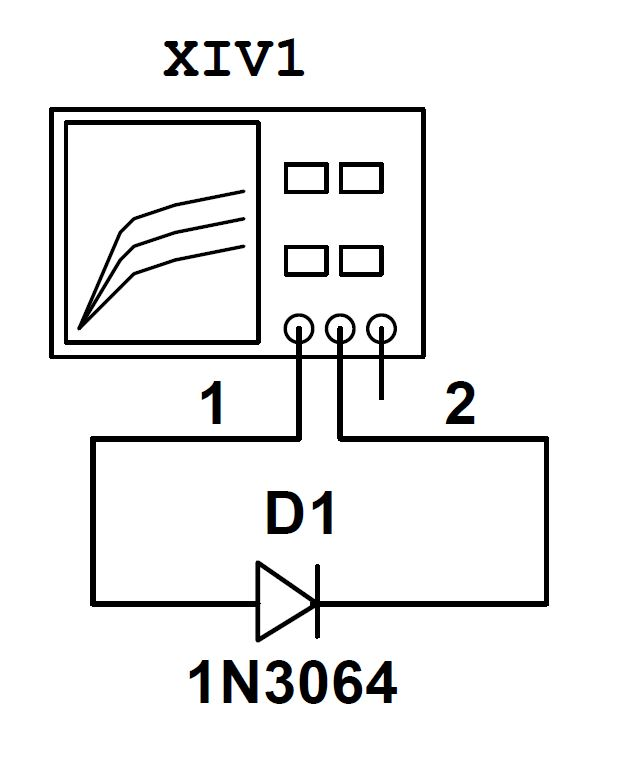
\includegraphics [width=40mm]{cap/8.JPG}
\caption{二极管的伏安特性测量电路图}
\label{DCirc}
\end {wrapfigure}

因此可以得到二极管的击穿电压为75V以上,反向漏电电流在100nA以下,两端加载0.7V正向偏压时通过的电流大约为1mA。

下面使用IV分析仪测量上述几个基本参数,如图\ref{DCirc}所示将二极管1N3064接入IV分析仪两端,将“Component”设置为“Dioxide”,作为初步的仿真测试,将电压测试设定为-200V -- +200V进行宽范围仿真,得到通过二极管的电流如图\ref{general}所示

\begin{figure}
\centering
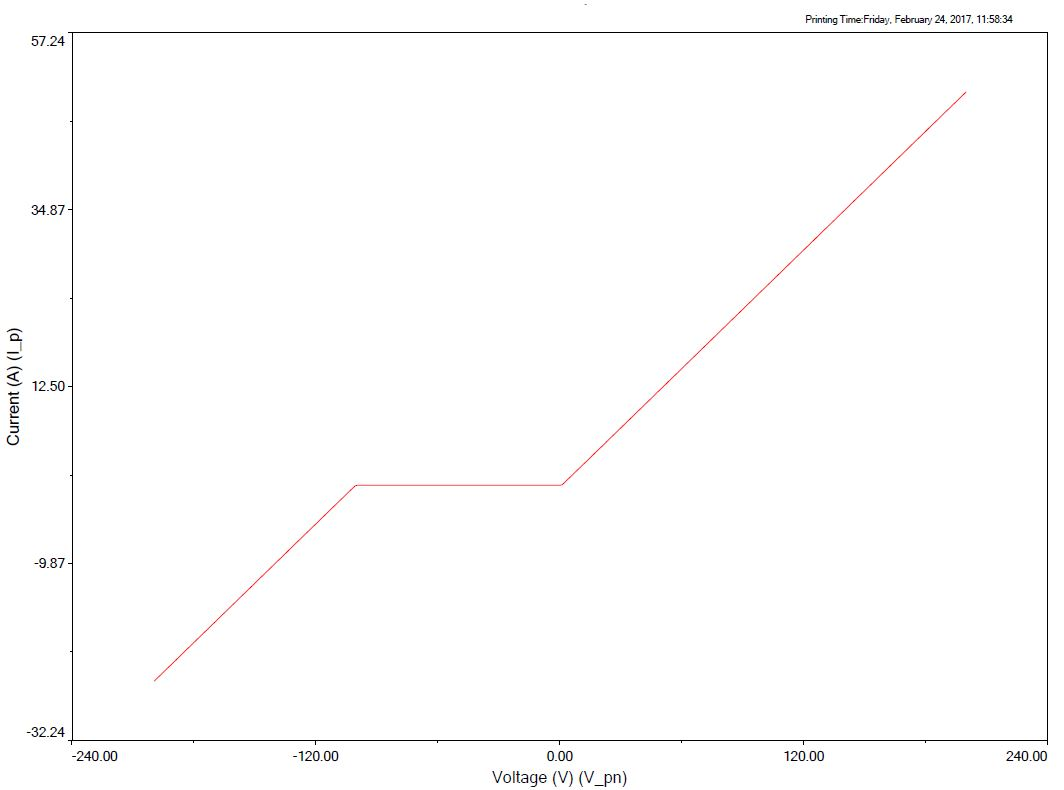
\includegraphics[width=\textwidth]{cap/16.JPG}
\caption{二极管伏安特性的宽范围测试图}
\label{general}

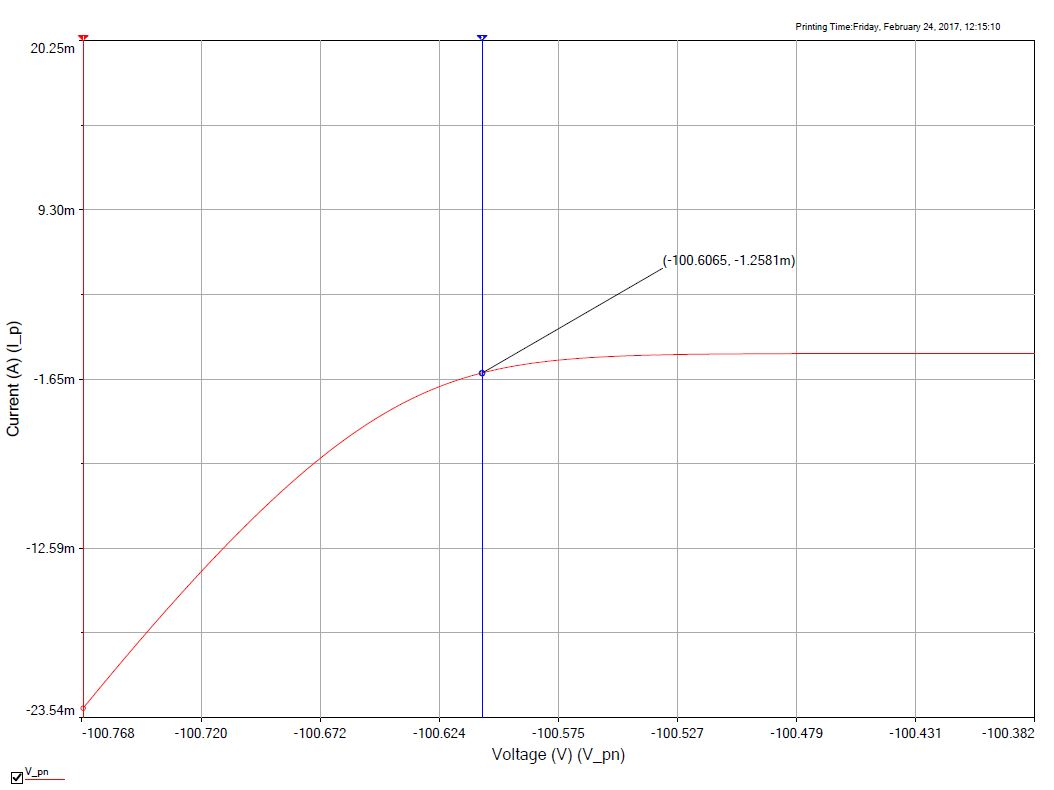
\includegraphics[width=\textwidth]{cap/18.JPG}
\caption{二极管反向击穿电压测试图}
\label{break}
\end{figure}
\begin{figure}
\centering
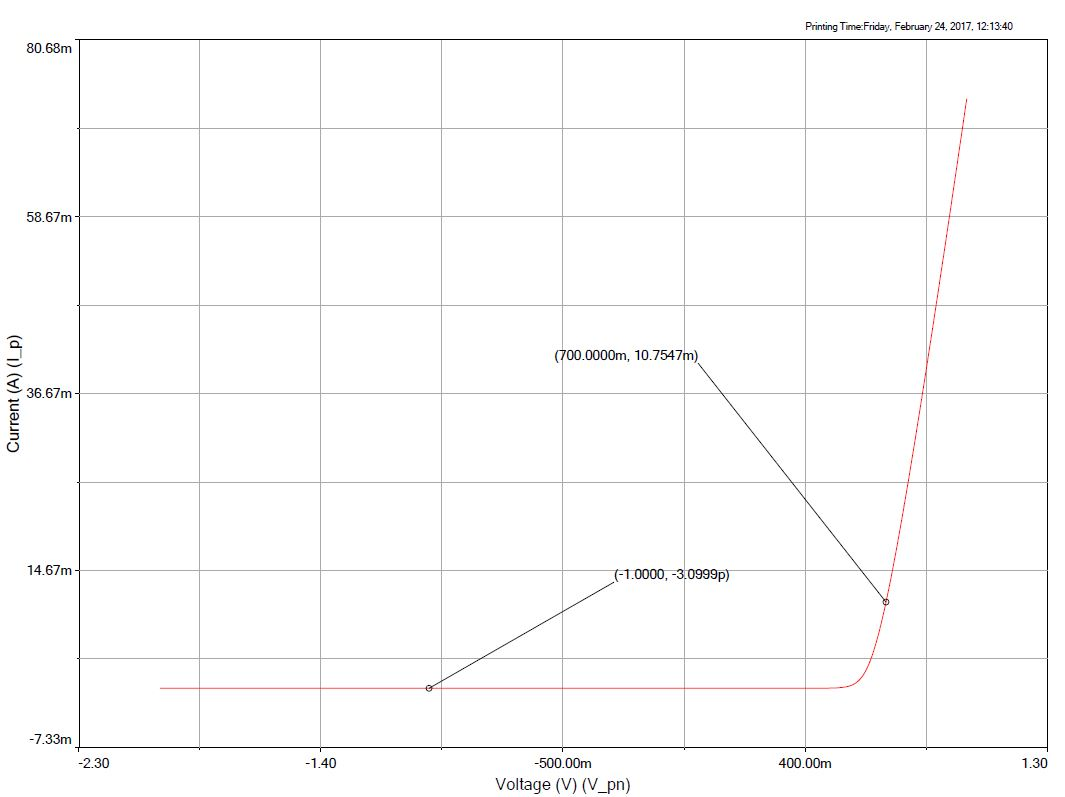
\includegraphics[width=\textwidth]{cap/15.JPG}
\caption{二极管导通电流和反向电流测试图}
\label{normal}

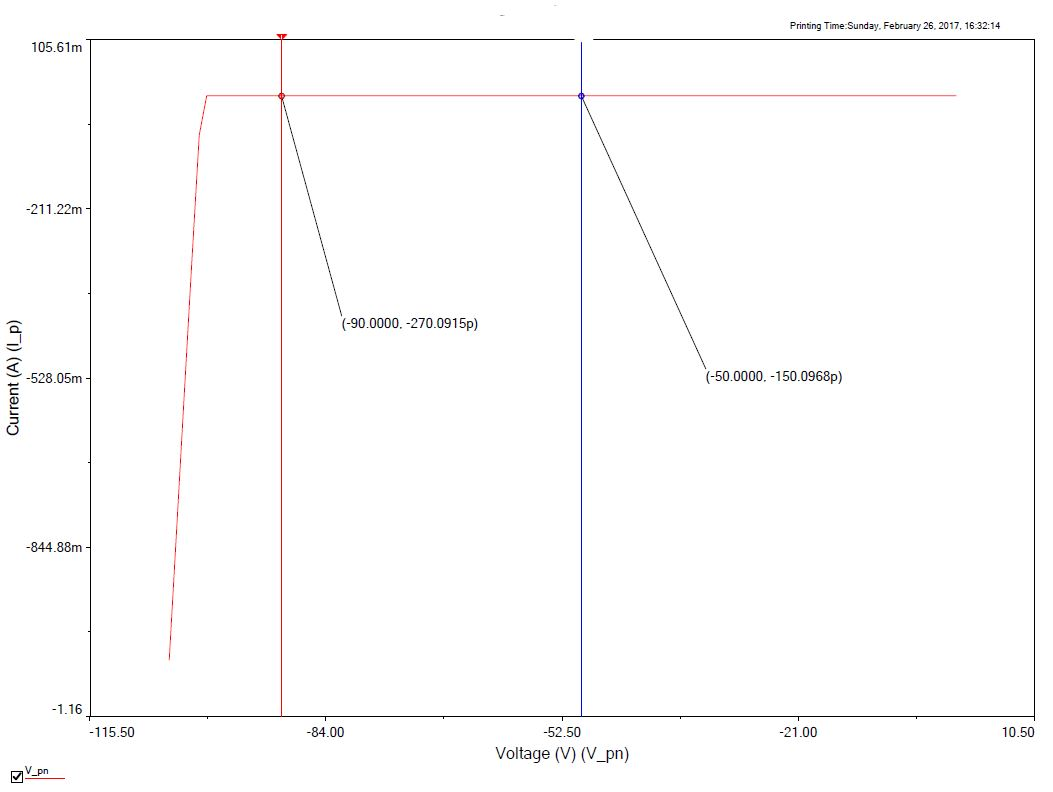
\includegraphics[width=\textwidth]{cap/19.JPG}
\caption{二极管反向电流测试图}
\label{normalR}

\end{figure}

从图\ref{general}可以看出,反向击穿的具体位置大约应在-100V附近,同时可以看出二极管截止和导通区域的大致位置,方便进一步的测量。

将IV分析仪的两端电压的变化区间设置为-120V -- -90V以便准确测量反向击穿电压,根据实验情况不断缩小测试范围以提高测试精度,可以得到IV分析仪的输出如图\ref{break}所示。

根据图\ref{break}的曲线变化形势可得,反向电压变化的转折点可以估算为-100V,电压大小高于数据手册中的-75V,符合数据手册中的要求

同理,将测试电压范围设为-5V -- 1V,测量题目中要求的反向电流和0.7V正向偏压是的导通电流,可以得到如图\ref{normal}所示的结果

从图\ref{normal}可以看到,二极管的反向电流在反向击穿前基本保持不变,在反向电压为-1V的时候约为3pA。另外,从图\ref{normalR}中可以看出,当反向电压上升到-50V甚至-90V时,反向电流仍为150pA和270pA,和1V时的反向电流略有上升,但均在1nA以下。和数据手册相比,仿真得到的效果要好一些,考虑是因为仿真模型没有受实际封装的影响等原因导致的 
\subsection{晶体管输出特性的测试}

\begin {wrapfigure}{r}{0pt}
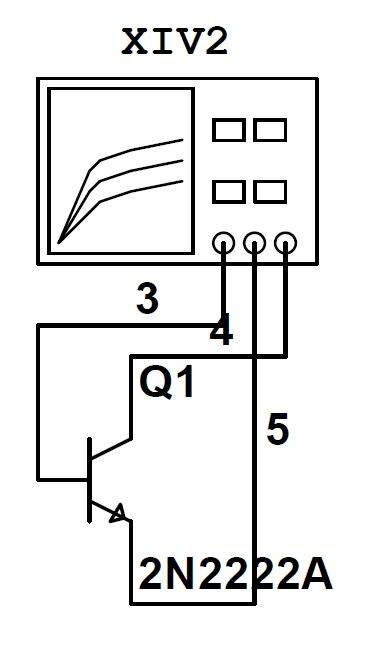
\includegraphics [width=20mm]{cap/9.JPG}
\caption{晶体管输出特性的测试电路图}
\label{TCirc}
\end {wrapfigure}
通过查阅相关手册,可以得到ZETEX公司生产的晶体管2N2222A的$\beta_{min}=100,\beta_{max}=300(@I_c=150\rm{mA})$,采用如图\ref{TCirc}的电路进行测试

将晶体管按照IV测试仪的指示接入IV测试仪,将“Component”设置为“BJT NPN”,将$I_b$设置为$0\rm{A} -- 10\rm{\mu A} $,$U_{ce}$设置为0V~10V进行宽范围测试,得到图\ref{Tgeneral}所示的结果 
\begin {figure}
\centering
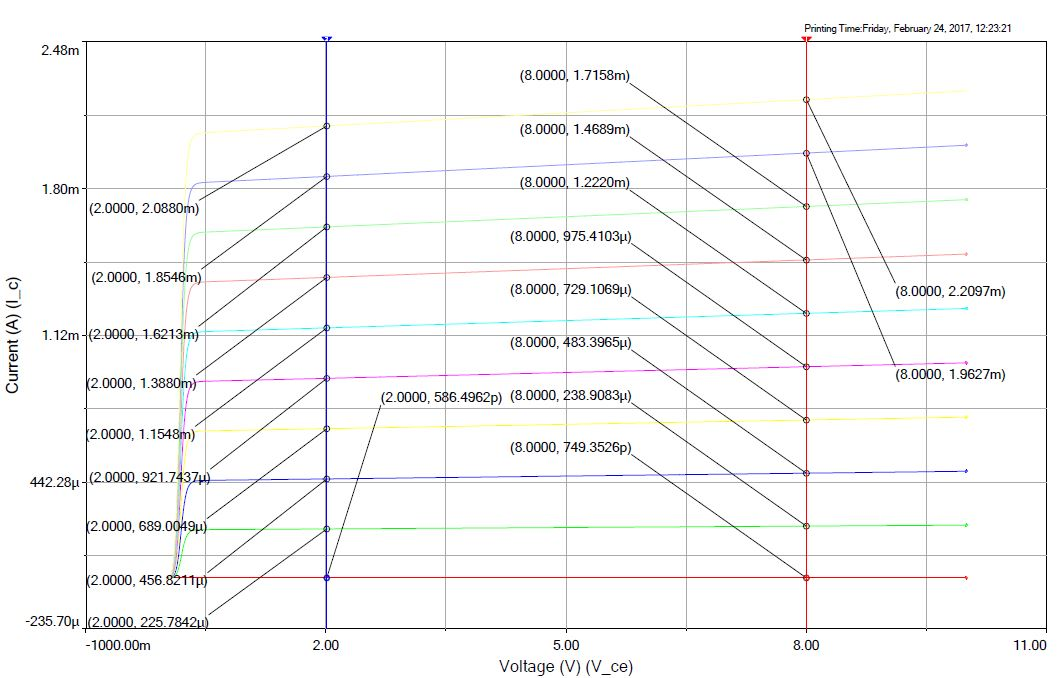
\includegraphics[width=\textwidth]{cap/17.JPG}
\caption{晶体管输出特性}
\label{Tgeneral}
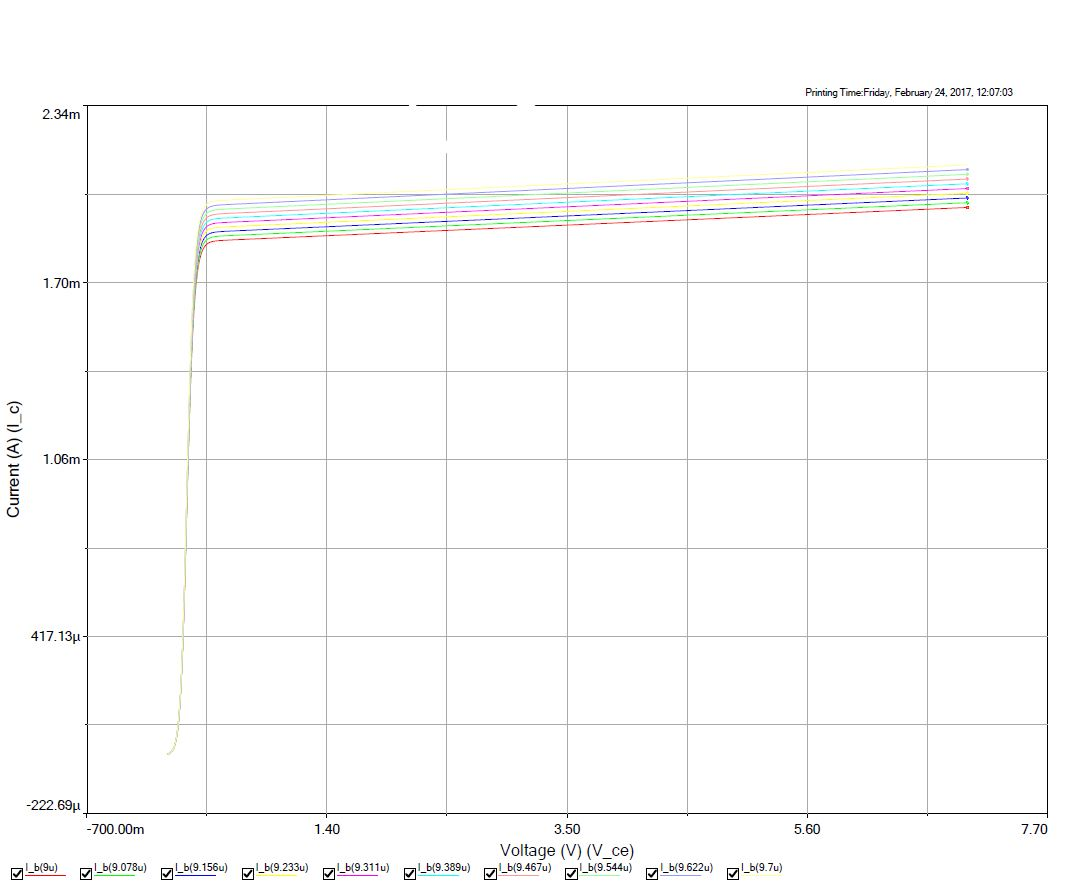
\includegraphics[width=\textwidth]{cap/2.JPG}
\caption{晶体管指定工作点放大系数的测量}
\label{micro}
\end{figure}
\begin{figure}
\centering
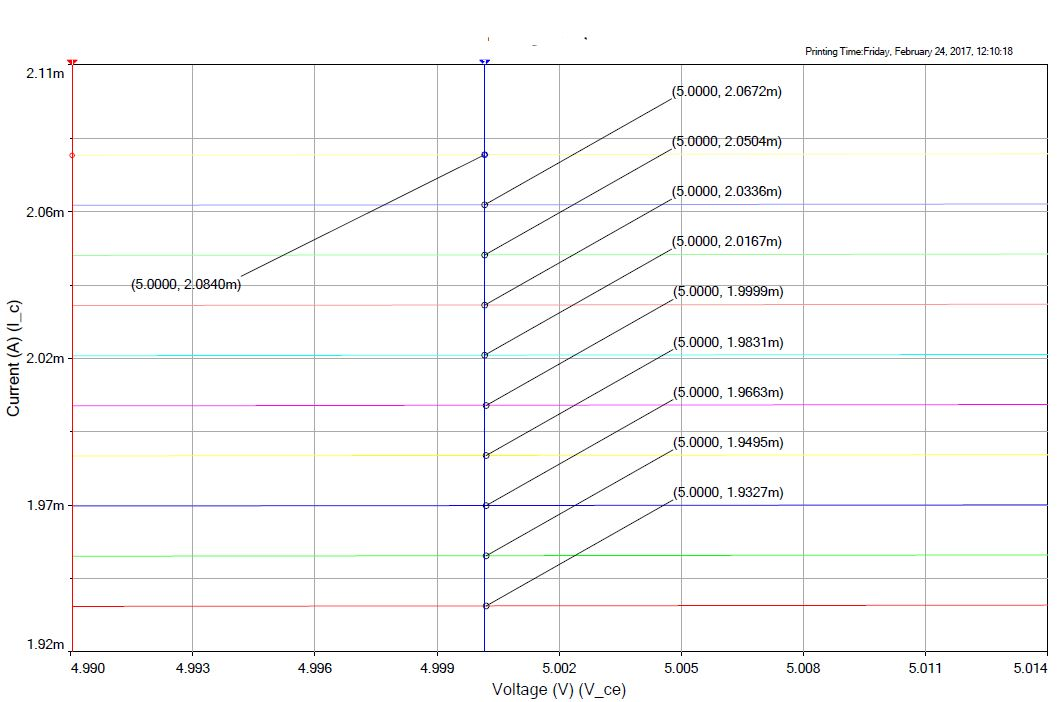
\includegraphics[width=\textwidth]{cap/4.JPG}
\caption{图\ref{micro}的指定工作点附近图像}
\label{large}
\end{figure}
\subsubsection{$\beta$变化情况的研究}
在图\ref{Tgeneral}中标识了在$U_{ce}=2\rm{V}$和$U_{ce}=8\rm{V}$下,$I_c$随着$I_b$的变化情况,具体来说可以总结为下表
\\

\begin{tabular}{|c|c|c|}
\hline
\tabincell{c}{$I_b/\rm{\mu A}$}& \tabincell{c}{$I_c/\rm{mA}@U_{ce}=2\rm{V}$}& \tabincell{c}{$I_c/\rm{mA}@U_{ce}=8\rm{V}$}\\
\hline
0.00&0.0005&0.0007 \\
\hline
1.11&0.2258 &0.2389 \\
\hline
2.22&0.4568 &0.4834 \\
\hline
3.33&0.6890 &0.7291 \\
\hline
4.44&0.9217 &0.9754 \\
\hline
5.56&1.1549 &1.2220 \\
\hline
6.67&1.3880 &1.4689 \\
\hline
7.78&1.6213 &1.7158 \\
\hline
8.89&1.8546 &1.9627 \\
\hline
10&2.0880 &2.2097 \\
\hline
\end{tabular}
\\

于是可以对两种情况下的$I_c$和$I_b$做直线拟合得到
$$I_c=209.06I_b-5.2456(\rm{\mu A})@U_{ce}=2\rm{V},R^2=1,\beta=209.06$$
$$I_c=221.24I_b-5.5308(\rm{\mu A})@U_{ce}=8\rm{V},R^2=1,\beta=221.24$$
进而可以得到结论,即$U_{ce}$越大,晶体管的$\beta$值越大,式中R为线性相关系数,下同

利用同样的方法,可以对$U_{ce}=5\rm{V},I_c=2\rm{mA}$的情况进行测试,通过之前的测试结果可以得到,晶体管的$\beta$值应在200左右,因此调整$I_b$在$10\rm{\mu A}$附近变化,得到图\ref{micro},对所求位置进行放大得到图\ref{large},标出数据得到下表\\ 

\begin{tabular}{|c|c|c|c|}
\hline
\tabincell{c}{$I_b/\rm{\mu A}$}& \tabincell{c}{$I_c/\rm{mA}@U_{ce}=5\rm{V}$}&\tabincell{c}{$I_b/\rm{\mu A}$}& \tabincell{c}{$I_c/\rm{mA}@U_{ce}=5\rm{V}$}\\
\hline
9.078&1.9327&9.156&1.9495\\
\hline
9.233&1.9663&9.311&1.9831\\
\hline
9.389&1.9999&9.467&2.0167\\
\hline
9.544&2.0336&9.622&2.0504\\
\hline
9.7&2.0672&&\\
\hline
\end{tabular}\\

利用同样的方法,可以得到在$U_{ce}=5\rm{V},I_c=2\rm{mA}$时,$\beta = \frac{\Delta I_c}{\Delta I_b}=215.48,\bar{\beta} = \frac{I_c}{I_b}=213,\bar{\beta}\approx \beta$可以认为晶体管还是比较理想的,另外和数据手册中给出的$100\le\beta\le300$也是符合的

\subsubsection{Early Voltage $V_A$的求取}
Early Voltage是一个用来描述晶体管工作特性的量。一般来说,作为理想情况,认为在晶体管处在放大区时$I_c$不随$U_{ce}$变化,然而实际情况下,$I_c$可认为随$U_{ce}$线性变化。由半导体物理的理论分析可以得到,$I_c-U_{ce}$直线簇的延长线交于同一点$(-V_A,I_0)$,其中$V_A$被定义为Early Voltage,显然,Early Voltage越大,直线簇的水平型越好。

设这些直线簇的斜率和截距为$k$和$b$,于是根据上面表述,$k-b$应满足线性关系,即$I_0=-kV_A+b$,整理可得
\begin{equation} \label{kb}
b=kV_A+I_0
\end{equation}
即可以通过拟合来得到$V_A$
参考图\ref{Tgeneral}可以得到曲线簇中的点坐标和$k,b$关系如下表所示\\

\begin{tabular}{|c|c|c|c|}
\hline
\tabincell{c}{$I_c/\rm{mA}@U_{ce}=2\rm{V}$}& \tabincell{c}{$I_c/\rm{mA}@U_{ce}=8\rm{V}$}&$k/\rm{(mA/V)}$&b/\rm{mA}$$\\
\hline
0.0005&0.0007&$3.33 \times 10^{-5}$&$4.33\times 10^{-4}$ \\
\hline
0.2258 &0.2389&$2.18 \times 10^{-3}$&$2.21\times 10^{-1}$ \\
\hline
0.4568 &0.4834&$4.43 \times 10^{-3}$&$4.48\times 10^{-1}$ \\
\hline
0.6890 &0.7291&$6.68 \times 10^{-3}$&$6.76\times 10^{-1}$ \\
\hline
0.9217 &0.9754&$8.95 \times 10^{-3}$&$9.04\times 10^{-1}$ \\
\hline
1.1549 &1.2220&$1.12 \times 10^{-2}$&$1.13\times 10^0$ \\
\hline
1.3880 &1.4689&$1.35 \times 10^{-2}$&$1.36\times 10^0$ \\
\hline
1.6213 &1.7158&$1.58 \times 10^{-2}$&$1.59\times 10^0$ \\
\hline
1.8546 &1.9627&$1.80 \times 10^{-2}$&$1.82\times 10^0$ \\
\hline
2.0880 &2.2097&$2.03 \times 10^{-2}$&$2.05\times 10^0$ \\
\hline
\end{tabular}

拟合可以得到$b=100.99k-9\times 10^{-5},R^2=0.99998$根据(\ref{kb})式可得,$V_A=100.99 \rm{V}$符合查阅相关资料得到的经典值100V

\section{二极管微变等效电路直流电压和交流电流的研究}
\subsection{直流电压的研究}
\begin {wrapfigure}{r}{0pt}
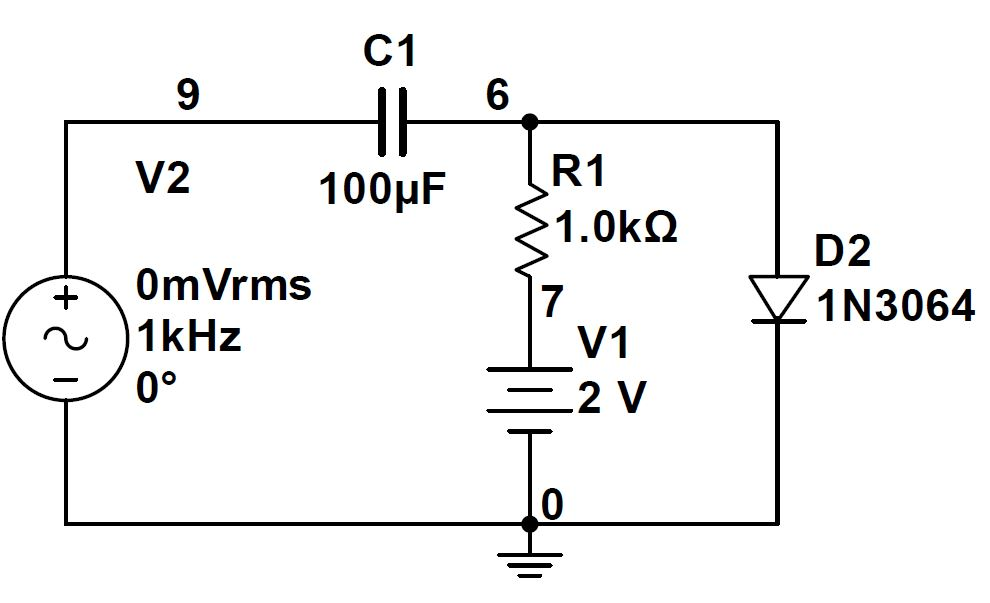
\includegraphics [width=60mm]{cap/10.JPG}
\caption{分析直流电压的电路图}
\label{DCV}
\end {wrapfigure}
如图\ref{DCV}所示为分析直流电压的电路图,因为只考虑直流成分,因此可以直接将交流电压幅值将为0。采用直流工作点分析对$R_1$进行扫描可以完成相关工作,如图\ref{DCP}所示,随着电阻值的增高,二极管上的直流电压逐渐减小,符合预期。最终随着$R_1$的逐渐增大,二极管两端的电压稳定在二极管的导通电压附近。从图中读出这个电压约为0.6-0.7V,符合第一节进行测量得到的结论和常识。


\subsection{交流电流的研究}

如图\ref{ACA}所示是分析交流电流的电路图。由于没有找到能比较简单直接分析交流成分的方式,因此采用这种方法进行分析。其中$R_2$是可变电阻,$XCP1$是电流探针,可以按照1V/mA的比例将电流转化为电压,$XSC1$是示波器, 因为关注交流成分,因此选择AC模式进行观测。逐个改变R2的阻值,可以得到点点对应的电压(即电流)值,利用数学软件进行作图可以得到图\ref{ACP}。从理论上分析,随着$R_2$的增大,通过$D_3$的直流电流逐渐减小。由二极管的微变等效电路模型可知,对应交流电流的动态电阻$r_g=\frac{U_T}{I_D}$因此动态电阻不断增大,通过$D_3$的交流电流逐渐减小,参考图\ref{ACP}可以验证其正确性。因为测量的数据点见下表。\\

\begin{tabular}{|c|c|c|c|c|c|c|c|}
\hline
$R/\Omega$&$i/\rm{mA}$&$R/\Omega$&$i/\rm{mA}$&$R/\Omega$&$i/\rm{mA}$&$R/\Omega$&$i/\rm{mA}$\\
\hline
1000&0.39295&950&0.4100&900&0.4306&850&0.4493\\
\hline
800&0.4721&750&0.4973&700&0.5251&650&0.5564\\
\hline
600&0.5918&550&0.6317&500&0.6774&450&0.7928\\
\hline
400&0.8777&350&0.9618&300&1.0467&250&1.1471\\
\hline
200&1.2694&150&1.4201&100&1.6089&50&1.8770\\
\hline
\end{tabular}

\begin{figure}
\centering
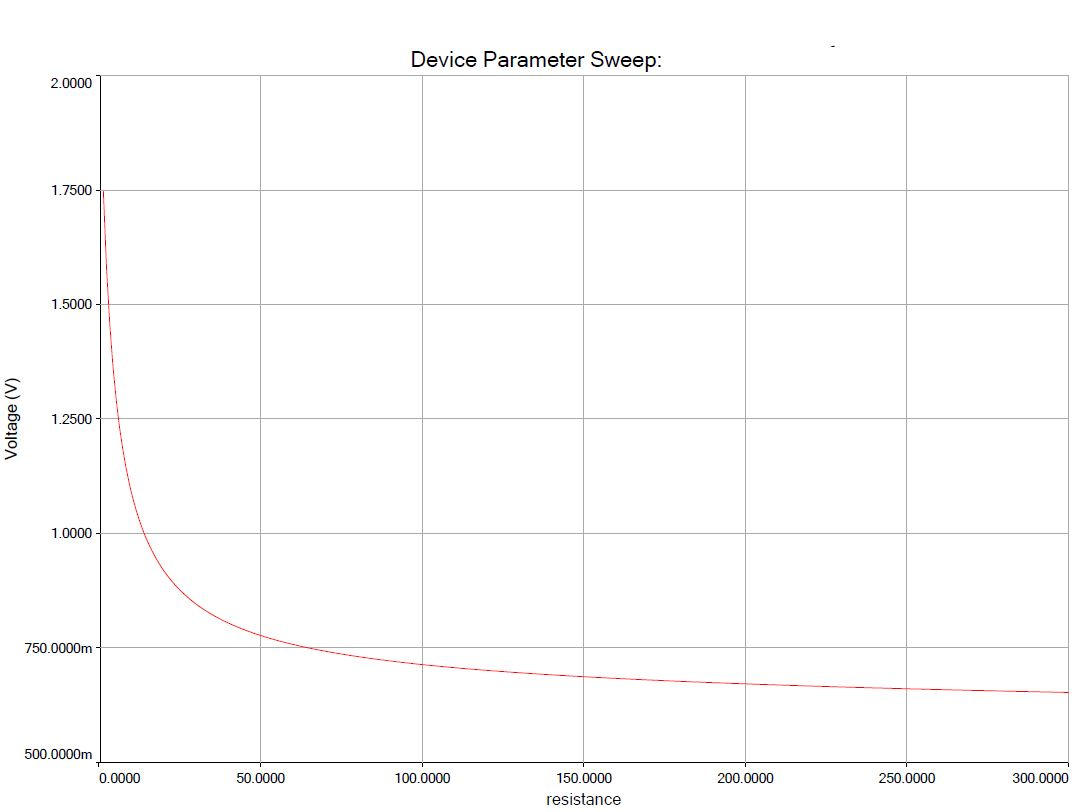
\includegraphics[width=\textwidth]{cap/3.JPG}
\caption{直流电压随电阻变化曲线}
\label{DCP}
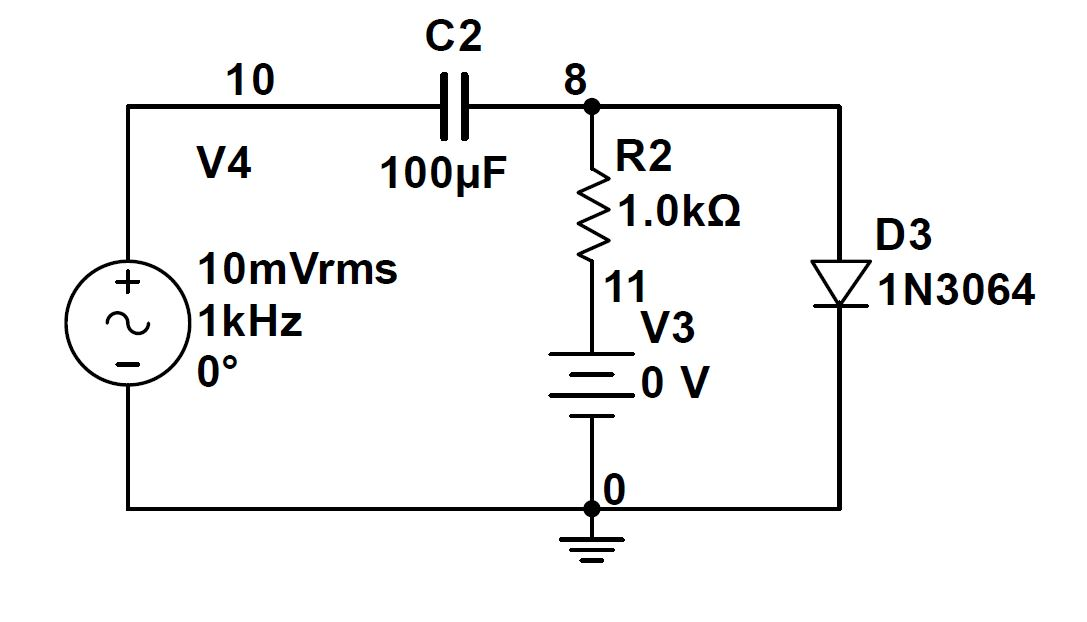
\includegraphics [width=\textwidth]{cap/11.JPG}
\caption{分析交流电压的电路图}
\label{ACA}
\end{figure}
\begin{figure}
\centering
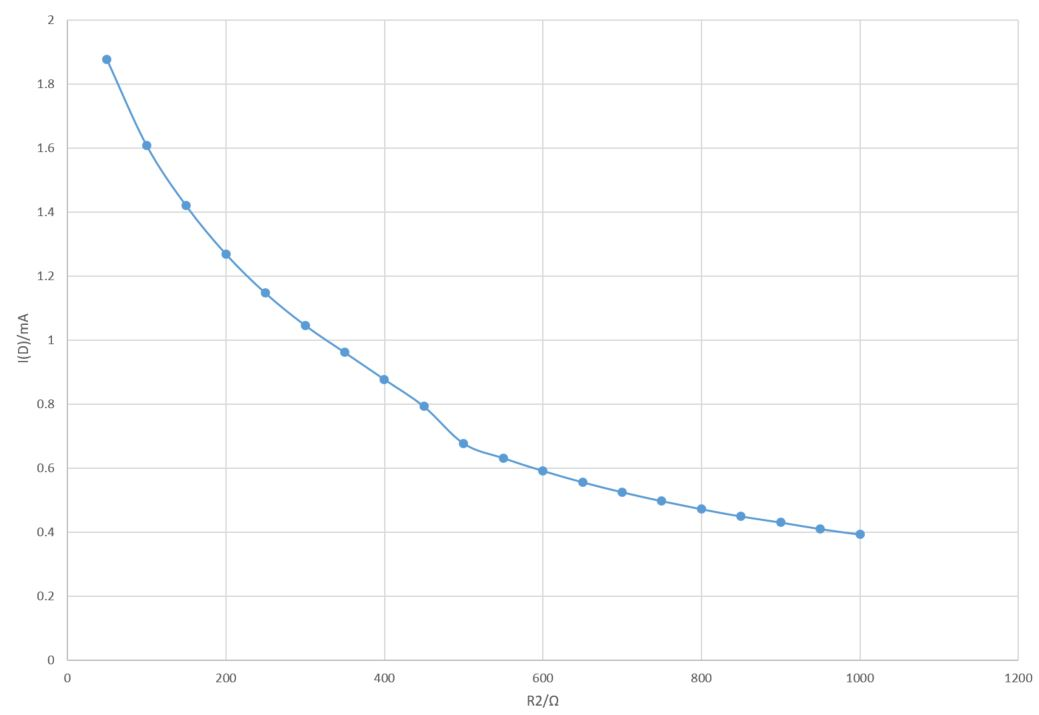
\includegraphics[width=\textwidth]{cap/21.JPG}
\caption{交流电压随电阻变化关系}
\label{ACP}
\end{figure}

\section{晶体管工作状态的研究}

\begin {wrapfigure}{r}{0pt}
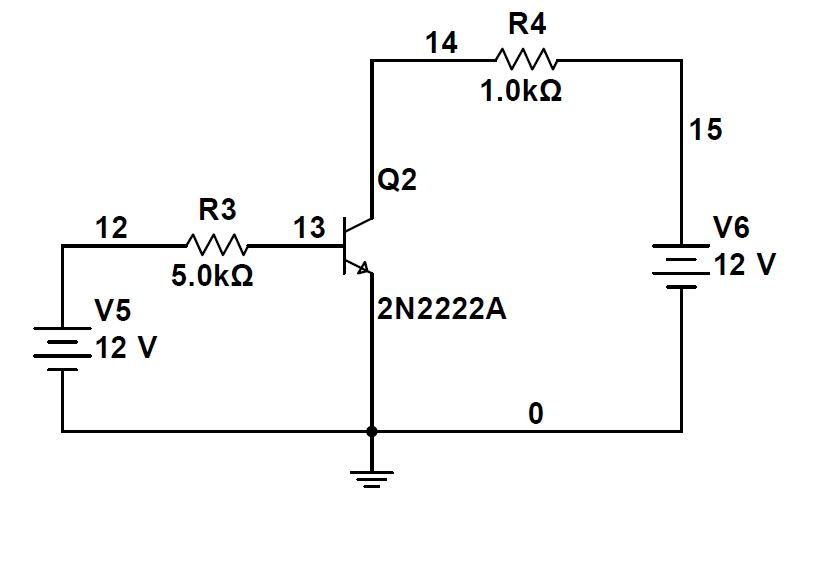
\includegraphics [width=60mm]{cap/12.JPG}
\caption{晶体管工作状态分析电路}
\label{BJT}
\end {wrapfigure}
图\ref{BJT}是分析晶体管工作状态的电路图。从理论上分析,随着$V_5$从0开始增大,首先使得BE间PN结导通,晶体管进入放大状态。之后随着$I_b,I_c$的增大,$V_{c}$下降至$V_b$以下,晶体管进入饱和状态。图\ref{simple}是其实际仿真得到的电路图,可以看出,在约0.6V时,晶体管进入放大状态,在0.969V附近,晶体管进入饱和状态。为了使得其中的效果更明显,将$V_{ce},V_{be},I_b,I_c$及$\frac{I_c}{I_b}$按照不同的比例绘制在了一张图上,如图\ref{complex}所示,其中黄色轨迹线为$\frac{I_c}{I_b}$的变化趋势,可以看出,在0.6V左右,$\frac{I_c}{I_b}$迅速上升并在之后相当长的区域内保持稳定,此时,$I_b,I_c$保持着相对稳定的上升状态标志晶体管进入放大状态;在0.969V附近,$\frac{I_c}{I_b}$迅速下降,$I_c$继续升高而$I_b$基本不变,标志晶体管进入饱和状态。曲线的变化均和前文的理论分析相符。

\begin{figure}
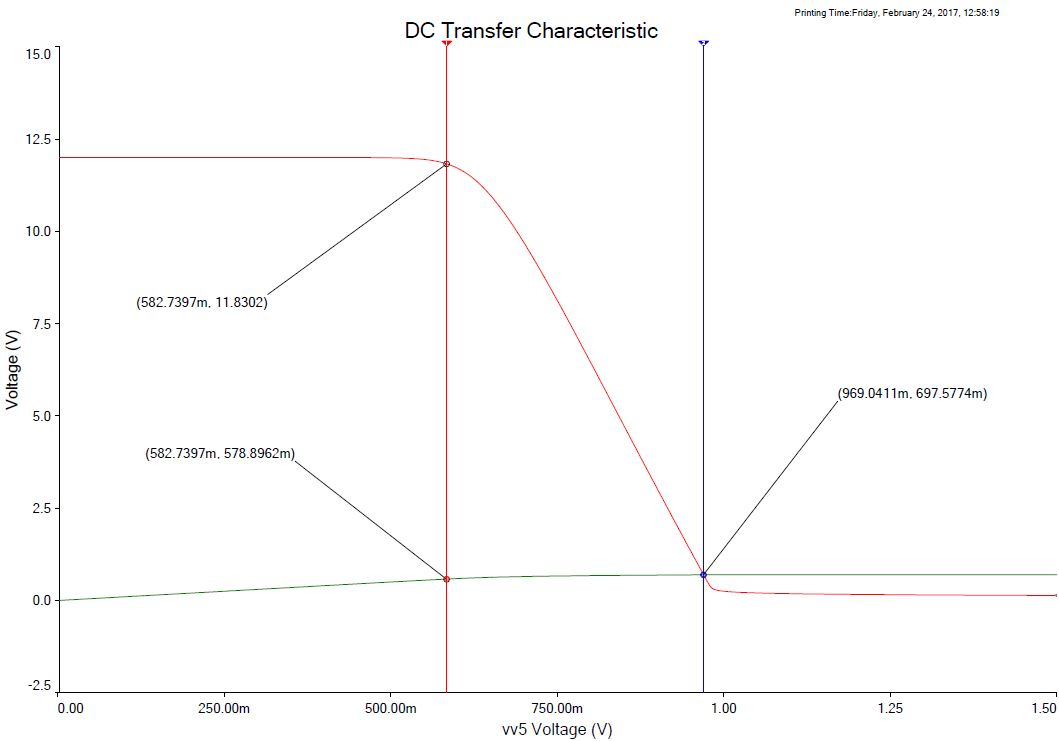
\includegraphics[width=\textwidth]{cap/20.JPG}
\caption{$V_{ce},V_{be}$变化曲线}
\label{simple}
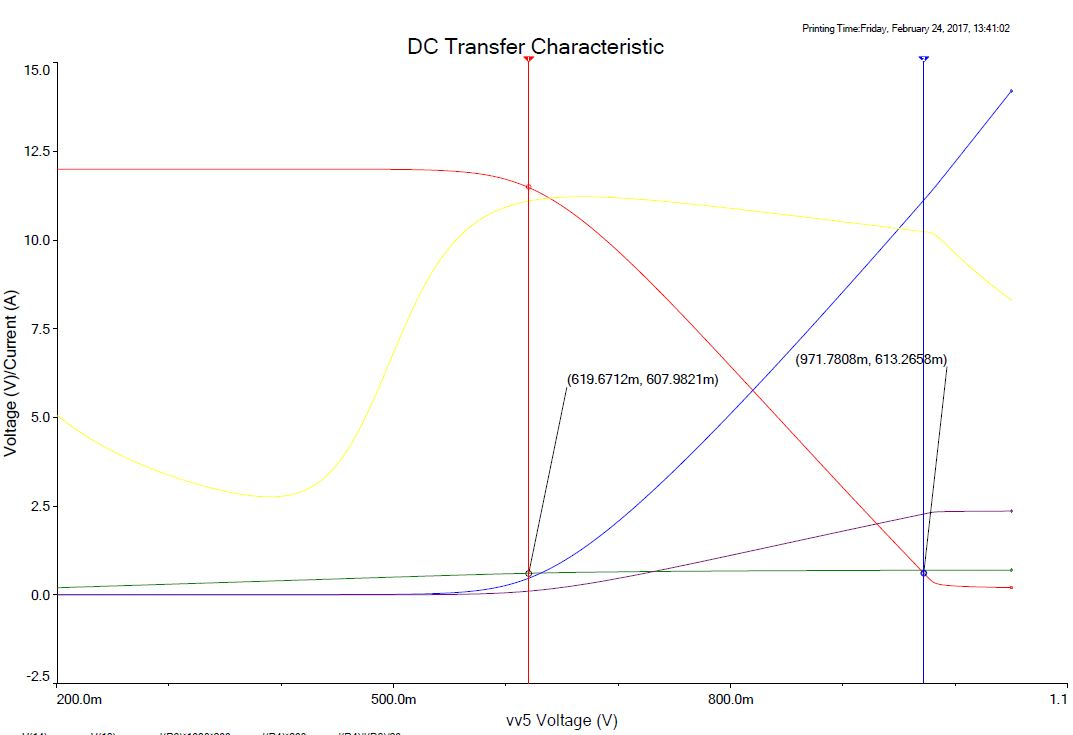
\includegraphics[width=\textwidth]{cap/14.JPG}
\caption{$V_{ce},V_{be},I_b,I_c$及$\frac{I_c}{I_b}$变化曲线}
\label{complex}
\end{figure}
\section{总结}
\subsection{仿真时遇到的问题}
仿真时对交流参数进行仿真的时候没有找到合适的自动仿真的选项,因此采用示波器手动读取相关参数。仿真时没有遇到其他问题
\subsection{收获}
客观了解了晶体管和二极管的工作特性,晶体管放大电路的各个可能的公共状态。同时测试了晶体管的$V_A$参数  

同时学习了Multisim的相关使用方法包括各种仿真参数模型的测试,电路的搭建和相关系数的测试等知识
\end {document}
